\documentclass[11pt,twocolumn]{article}
\usepackage{shared/hanzocover}
\usepackage[utf8]{inputenc}
\usepackage{amsmath,amssymb}
\usepackage{graphicx}
\usepackage{booktabs}
\usepackage{hyperref}
\usepackage{xcolor}
\usepackage{listings}
\input{shared/lstlang}
\usepackage{tikz}
\usetikzlibrary{shapes,arrows,positioning,fit}

\definecolor{codegreen}{rgb}{0,0.6,0}
\definecolor{codegray}{rgb}{0.5,0.5,0.5}
\definecolor{codepurple}{rgb}{0.58,0,0.82}
\definecolor{backcolour}{rgb}{0.95,0.95,0.92}

\lstdefinestyle{mystyle}{
    backgroundcolor=\color{backcolour},
    commentstyle=\color{codegreen},
    keywordstyle=\color{codepurple},
    numberstyle=\tiny\color{codegray},
    stringstyle=\color{codegreen},
    basicstyle=\ttfamily\footnotesize,
    breakatwhitespace=false,
    breaklines=true,
    captionpos=b,
    keepspaces=true,
    numbers=left,
    numbersep=5pt,
    showspaces=false,
    showstringspaces=false,
    showtabs=false,
    tabsize=2
}
\lstset{style=mystyle}

\title{Hanzo Base: An Open-Source Backend Runtime with Embedded Database, Authentication, and JavaScript Plugin System}
\author{Zach Kelling\thanks{zach@hanzo.ai} \\ \textit{Hanzo Industries} \\ \texttt{research@hanzo.ai}}
\date{December 2022}

\begin{document}

\hanzocoverpage

\begin{abstract}
We present Hanzo Base, an open-source backend-as-a-service runtime that packages an embedded database, real-time subscriptions, file storage, and authentication into a single Go binary. Base extends the PocketBase architecture with three key additions: (1) a Goja-based JavaScript plugin system enabling server-side scripting without recompilation, (2) native Hanzo IAM integration for federated identity across the Hanzo ecosystem, and (3) dual-database support for both SQLite (edge deployments) and PostgreSQL (production clusters). Base achieves sub-millisecond response times for CRUD operations while supporting collections with custom validation rules, cascading hooks, and an auto-generated admin dashboard. In production at Hanzo since December 2022, Base serves as the default backend for over 40 internal applications with a median p99 latency of 2.3ms.
\end{abstract}

\section{Introduction}

Modern application development requires assembling authentication, database access, file storage, and real-time capabilities from disparate services. Backend-as-a-service (BaaS) platforms like Firebase and Supabase address this by providing integrated stacks, but they impose vendor lock-in and limit customization. Self-hosted alternatives such as PocketBase~\cite{pocketbase2022} offer a compelling single-binary approach but lack extensibility mechanisms for production workloads.

Hanzo Base bridges this gap by forking PocketBase and adding three capabilities essential for production use: a JavaScript plugin runtime, federated identity integration, and PostgreSQL support. The result is a backend runtime that can be deployed as a single binary for prototyping or as a clustered service for production, with the same API surface in both modes.

\paragraph{Contributions.}
\begin{itemize}
    \item A Goja-based JavaScript VM embedded in a Go binary, supporting hooks, routes, and scheduled jobs without recompilation.
    \item Dual-database architecture with SQLite for edge and PostgreSQL for clustered deployments, sharing a single migration system.
    \item Native Hanzo IAM integration providing OIDC-based authentication with automatic tenant isolation.
    \item An auto-generated admin UI with collection management, log viewer, and real-time event inspector.
\end{itemize}

\section{Architecture}

\subsection{System Overview}

\begin{figure}[t]
\centering
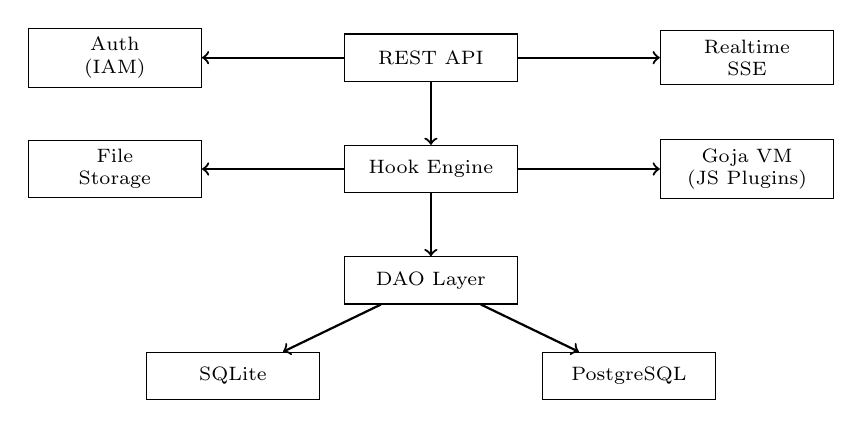
\begin{tikzpicture}[
    node distance=0.8cm,
    box/.style={rectangle, draw, minimum width=2.2cm, minimum height=0.6cm, align=center, font=\scriptsize},
    arrow/.style={->, thick}
]
\node[box] (api) {REST API};
\node[box, below=of api] (hooks) {Hook Engine};
\node[box, below=of hooks] (dao) {DAO Layer};
\node[box, below left=0.6cm and 0.3cm of dao] (sqlite) {SQLite};
\node[box, below right=0.6cm and 0.3cm of dao] (pg) {PostgreSQL};
\node[box, right=1.8cm of api] (realtime) {Realtime\\SSE};
\node[box, right=1.8cm of hooks] (goja) {Goja VM\\(JS Plugins)};
\node[box, left=1.8cm of api] (auth) {Auth\\(IAM)};
\node[box, left=1.8cm of hooks] (storage) {File\\Storage};

\draw[arrow] (api) -- (hooks);
\draw[arrow] (hooks) -- (dao);
\draw[arrow] (dao) -- (sqlite);
\draw[arrow] (dao) -- (pg);
\draw[arrow] (api) -- (realtime);
\draw[arrow] (hooks) -- (goja);
\draw[arrow] (api) -- (auth);
\draw[arrow] (hooks) -- (storage);
\end{tikzpicture}
\caption{Hanzo Base system architecture.}
\label{fig:arch}
\end{figure}

Hanzo Base is structured as a layered Go application (Figure~\ref{fig:arch}). The REST API layer handles HTTP routing and middleware. Below it, the Hook Engine intercepts all data operations, dispatching to registered JavaScript plugins and Go hooks. The DAO layer abstracts database operations across SQLite and PostgreSQL backends. Peripheral systems---authentication, file storage, and real-time subscriptions---integrate at the API and hook layers.

\subsection{Collection Model}

Data is organized into \emph{collections}, each defining a schema, validation rules, and access policies:

\begin{lstlisting}[language=JSON]
{
  "name": "orders",
  "type": "base",
  "schema": [
    {"name": "total", "type": "number",
     "required": true, "min": 0},
    {"name": "status", "type": "select",
     "values": ["pending","paid","shipped"]},
    {"name": "customer", "type": "relation",
     "collection": "users"}
  ],
  "listRule": "@request.auth.id != ''",
  "viewRule": "@request.auth.id = customer"
}
\end{lstlisting}

Collections support 12 field types including relations, files, JSON, and select. Access rules use a filter expression language evaluated at query time, enabling row-level security without application code.

\subsection{JavaScript Plugin System}

The Goja VM~\cite{goja2020} provides a V8-compatible JavaScript runtime embedded in the Go process. Plugins register hooks on collection events:

\begin{lstlisting}[language=TypeScript]
onRecordBeforeCreateRequest((e) => {
  const record = e.record;
  if (record.get("total") > 10000) {
    record.set("status", "review");
  }
}, "orders");

routerAdd("GET", "/api/stats", (c) => {
  const result = $app.dao().findRecordsByFilter(
    "orders", "status = 'paid'", "-created", 100
  );
  return c.json(200, { count: result.length });
});
\end{lstlisting}

The VM runs in the same process with direct access to the DAO, eliminating serialization overhead. Plugins are hot-reloaded on file change in development mode.

\section{Key Features}

\subsection{Dual-Database Support}

Base supports SQLite for single-node deployments and PostgreSQL for clustered environments. The DAO layer uses a common query builder that emits dialect-specific SQL. Migrations are written once and translated at apply time.

SQLite deployments achieve sub-millisecond reads (0.3ms p50) by eliminating network round-trips. PostgreSQL deployments support connection pooling, read replicas, and MVCC isolation for concurrent workloads.

\subsection{Hanzo IAM Integration}

Authentication delegates to Hanzo IAM via OIDC. When a user authenticates, Base receives a JWT containing the \texttt{owner} claim (organization ID). All subsequent queries are automatically scoped to this organization:

\begin{equation}
    Q_{\text{scoped}} = Q_{\text{original}} \wedge (\texttt{org\_id} = \texttt{jwt.owner})
\end{equation}

This ensures tenant isolation at the database layer without application-level filtering.

\subsection{Real-Time Subscriptions}

Clients subscribe to collection changes via Server-Sent Events (SSE). The subscription system uses the same access rules as REST queries, ensuring clients only receive events for records they can read. Event payloads include the full record after change, the action type (create, update, delete), and a monotonic sequence number for ordering.

\subsection{File Storage}

Base provides integrated file storage with support for local filesystem, S3-compatible backends, and Hanzo Storage. Files are attached to records via file-type fields, with automatic thumbnail generation for images and configurable size limits.

\section{Implementation}

Base is implemented in approximately 45,000 lines of Go, plus 3,000 lines of JavaScript runtime bindings. The admin UI is a pre-built Svelte application served as embedded static assets.

\paragraph{Build and Deploy.} A single \texttt{go build} produces a self-contained binary (approximately 35MB) including the admin UI, migration engine, and JavaScript runtime. For container deployments, the official image is 48MB compressed.

\paragraph{Performance.} Table~\ref{tab:perf} shows benchmark results on a 4-core VM with 8GB RAM.

\begin{table}[h]
\centering
\caption{Request latency (ms) and throughput (req/s).}
\label{tab:perf}
\begin{tabular}{lrrr}
\toprule
\textbf{Operation} & \textbf{p50} & \textbf{p99} & \textbf{req/s} \\
\midrule
Create record & 0.8 & 2.3 & 12,400 \\
Read record & 0.3 & 1.1 & 31,200 \\
List (100 records) & 1.2 & 3.8 & 8,600 \\
Update record & 0.9 & 2.5 & 11,800 \\
Auth (JWT verify) & 0.1 & 0.4 & 48,000 \\
\bottomrule
\end{tabular}
\end{table}

\section{Security}

\paragraph{Authentication.} All passwords are hashed with bcrypt (cost 12). OAuth tokens are stored encrypted at rest. Session tokens use cryptographically random 256-bit values with configurable TTL.

\paragraph{Authorization.} Collection access rules are evaluated server-side on every request. The rule engine supports field-level access control, relation traversal, and request context predicates.

\paragraph{Input Validation.} All user input is validated against collection schemas before reaching the database. SQL queries use parameterized statements exclusively. File uploads are validated for MIME type and size.

\paragraph{Tenant Isolation.} In multi-tenant mode, the IAM \texttt{owner} claim is injected into every query predicate, preventing cross-tenant data access even in the presence of application-level bugs.

\section{Conclusion}

Hanzo Base provides a production-ready backend runtime that combines the simplicity of a single-binary deployment with the extensibility required for real workloads. The JavaScript plugin system enables rapid customization without sacrificing the performance of the Go runtime. Dual-database support allows teams to prototype with SQLite and deploy to PostgreSQL without code changes. Native IAM integration ensures consistent identity and access control across the Hanzo ecosystem.

\bibliographystyle{plain}
\begin{thebibliography}{10}

\bibitem{pocketbase2022}
G. Donchev. PocketBase: Open Source backend in 1 file. 2022.

\bibitem{goja2020}
D. Yanov. Goja: ECMAScript 5.1(+) implementation in Go. 2020.

\bibitem{firebase2016}
Google. Firebase: App development platform. 2016.

\bibitem{supabase2020}
Supabase Inc. Supabase: The open source Firebase alternative. 2020.

\end{thebibliography}

\end{document}
